
\subworkpkg{1.4}

%% Tasks

%% A. Using methods based on statistical data and/or empirical
%% relationships (like, for instance, the ones presented in Refs. [1]
%% and [2]), define the preliminary mass and power budgets for the
%% spacecraft, i.e.  the mass and power distribution among all the
%% relevant subsystems. Pay particular attention to the definition of
%% proper design margins in your budgets.

%% B. Based on the information gathered so far, roughly sketch at
%% least three different preliminary architectures of the spacecraft
%% with its main components (e.g. antennae, solar arrays, batteries,
%% nuclear generator, payload units, external skin). Draft at least
%% one of these preliminary sketches as a CATIA drawing.

%% C. For each one of the proposed preliminary architectures, estimate
%% the vehicle MMOI (Mass Moment of Inertia) both for the deployed and
%% un-deployed state.  Deliverables

%% D1.4.1. Tables showing the preliminary mass and power budgets for
%% the spacecraft.

\deliverable{1.4.1}
Data was obtained from tables from
\cite[p. 589,590]{brown2002elements} for planetary spacecraft and
previous tasks.

The total on-orbit dry mass is

\[ m = 1100\mathrm{kg} \]

The minimum mass contingency for this class of spacecraft and stage of
design 30\%. This works out to a total on-orbit dry mass of 950kg.

Subsystem on-orbit drymass as percentages of total and absolute with
contingency margin removed are the following

\begin{center}
\begin{tabular}{rl}
Structure & $26\% \approx 290\mathrm{kg} - 86\mathrm{kg}$ \\
Thermal & $3\% \approx 33\mathrm{kg} - 9.9\mathrm{kg}$ \\
ACS & $9\% \approx 99\mathrm{kg} - 30\mathrm{kg}$ \\
Power & $19\% \approx 210\mathrm{kg} - 63\mathrm{kg}$ \\
Cabling & $7\% \approx 77\mathrm{kg} - 23\mathrm{kg}$ \\
Propulsion & $13\% \approx 140\mathrm{kg} - 43\mathrm{kg}$ \\
Telecom & $6\% \approx 66\mathrm{kg} - 20\mathrm{kg}$ \\
CDS & $6\% \approx 66\mathrm{kg} - 20\mathrm{kg}$ \\
Payload & $11\% \approx 120\mathrm{kg} - 36\mathrm{kg}$ \\
\end{tabular}
\end{center}

Total power usage is $P \approx 485{W}$.

The minimum power contingency is 90\%. Subsystem power allocation
estimates as percentages of subsystem total ($P_\mathrm{subsystems} =
P - P_\mathrm{payload} \approx 435\mathrm{W}$) and absolute with
contingency margin removed

\begin{center}
\begin{tabular}{rl}
Thermal control & $28\% \approx 120\mathrm{W} - 110\mathrm{W}$ \\
Attitude control & $20\% \approx 87\mathrm{W} - 78\mathrm{W}$ \\
Power & $10\% \approx 44\mathrm{W} - 39\mathrm{W}$ \\
CDS & $17\% \approx 74\mathrm{W} - 67\mathrm{W}$ \\
Communications & $23\% \approx 100\mathrm{W} - 90\mathrm{W}$ \\
Propulsion & $1\% \approx 4.4\mathrm{W} - 3.9\mathrm{W}$ \\
Mechanisms & $1\% \approx 4.4\mathrm{W} - 3.9\mathrm{W}$ \\
\end{tabular}
\end{center}

The launch vehicle adapter mass is given by

\[ M_{\mathrm{adapter}} = 0.0755 M_{\mathrm{launch}} + 50 \]


%% D1.4.2. Sketches of different optional preliminary spacecraft
%% architectures.

\deliverable{1.4.2}

%% D1.4.3. CATIA drawing of at least one preliminary spacecraft
%% architecture.

The first optional design was a circular satellite with a radius of
\SI{3.5}{m} and a height of \SI{4}{m} as seen in
figure \ref{sketch1}. On the bottom side of the satellite, the main
thruster and the payload are attached. This is because the payload
only needs to work when the thruster is turned of. On the top side of
the satellite, the location of the communication antennae is indicated
with a triangle. For this configuration, a nuclear power system is
used that is indicated with balloon 1. this will tilt outwards when
the satellite is being deployed. This is because the nuclear power
unit produces a lot of heat.

\begin{figure}[h!]
  \centering
  \includegraphics[angle=90, scale=0.25]{cylindrical}
  \caption{Cylindrical configuration}
  \label{sketch1}
\end{figure}

A next possible configuration is a cuboid with
dimensions \SI{2.5}{m}, \SI{3.5}{m}, and \SI{4.4}{m}. The undeployed
state can be seen in figure \ref{sketch2}. On the bottom view, the
thruster and the payload are attached. with the payload indicated as
balloon 1 and the thruster as balloon 2. On the side view the
undeployed solar panels are visible. On the top view is the location
of the antennae indicated with a triangle.
\begin{figure}[ht]
  \centering
  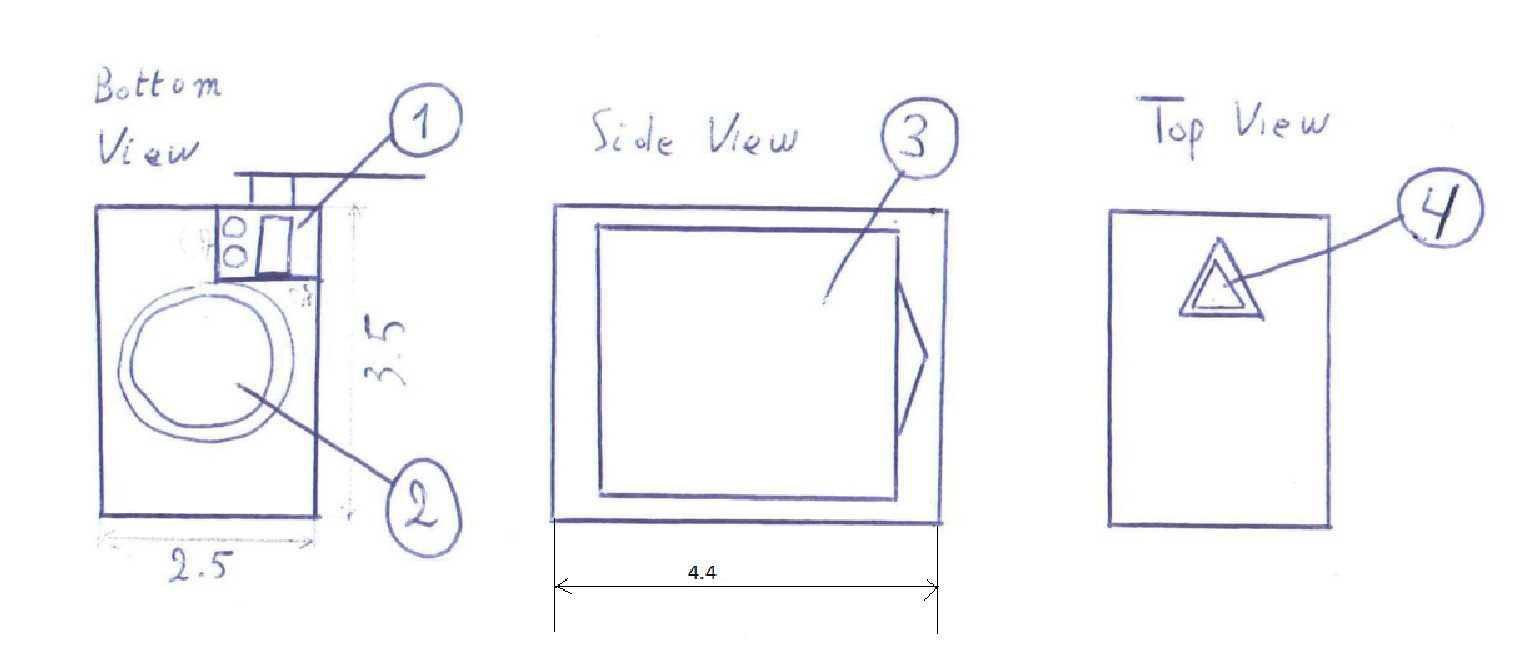
\includegraphics[width=\textwidth]{boxundeployed}
  \caption{undeployed state of cuboid shape}
  \label{sketch2}
\end{figure}

The deployed state can be seen in figures \ref{sketch3} and
\ref{sketch3-1}. The difference is that the folded solar panels are
now unfolded. From the reference data it was found a solar panel area
of \SI{60}{m^2} is needed. This results in 12 panels with dimensions
$\SI{3}{m}\cdot\SI{3.33}{m}$ equally distributed over the two sides.

\begin{figure}[ht]
  \centering
  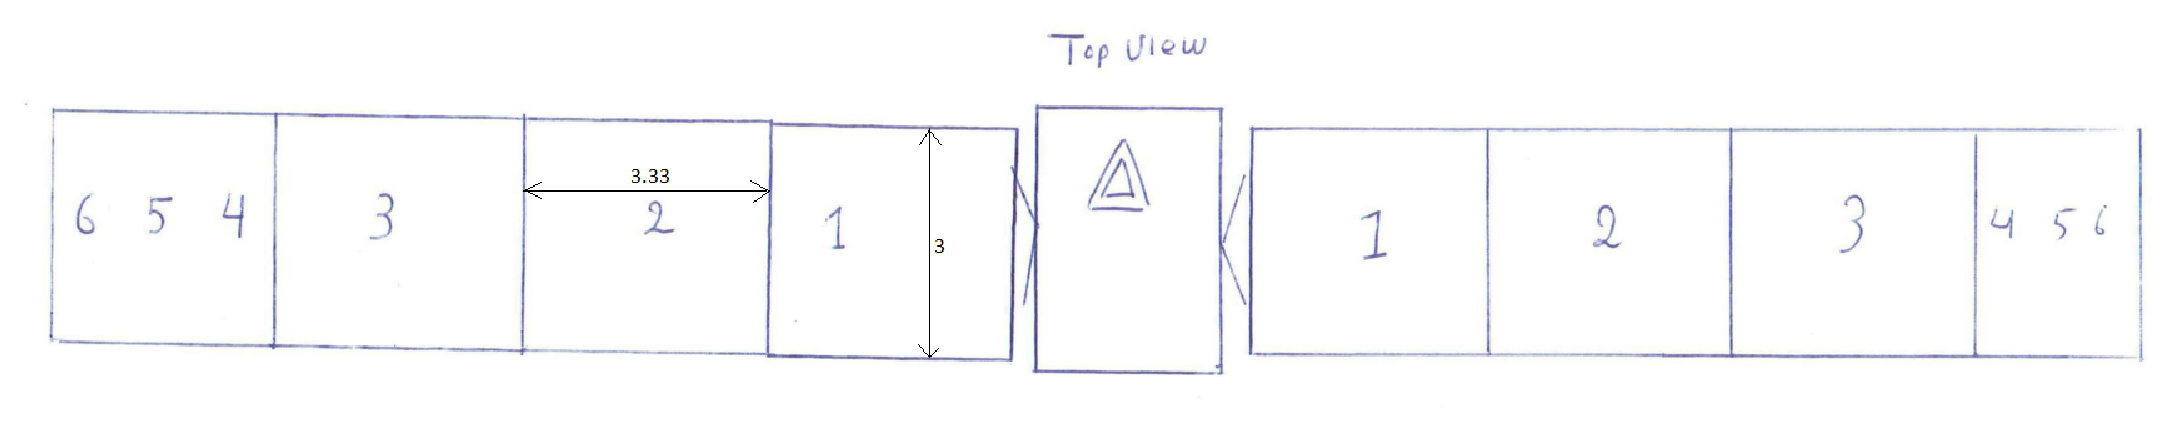
\includegraphics[width=\textwidth]{boxdeployed}
  \caption{deployed state of cuboid shape}
  \label{sketch3}
\end{figure}

\deliverable{1.4.3}

\begin{figure}[H]
  \centering
  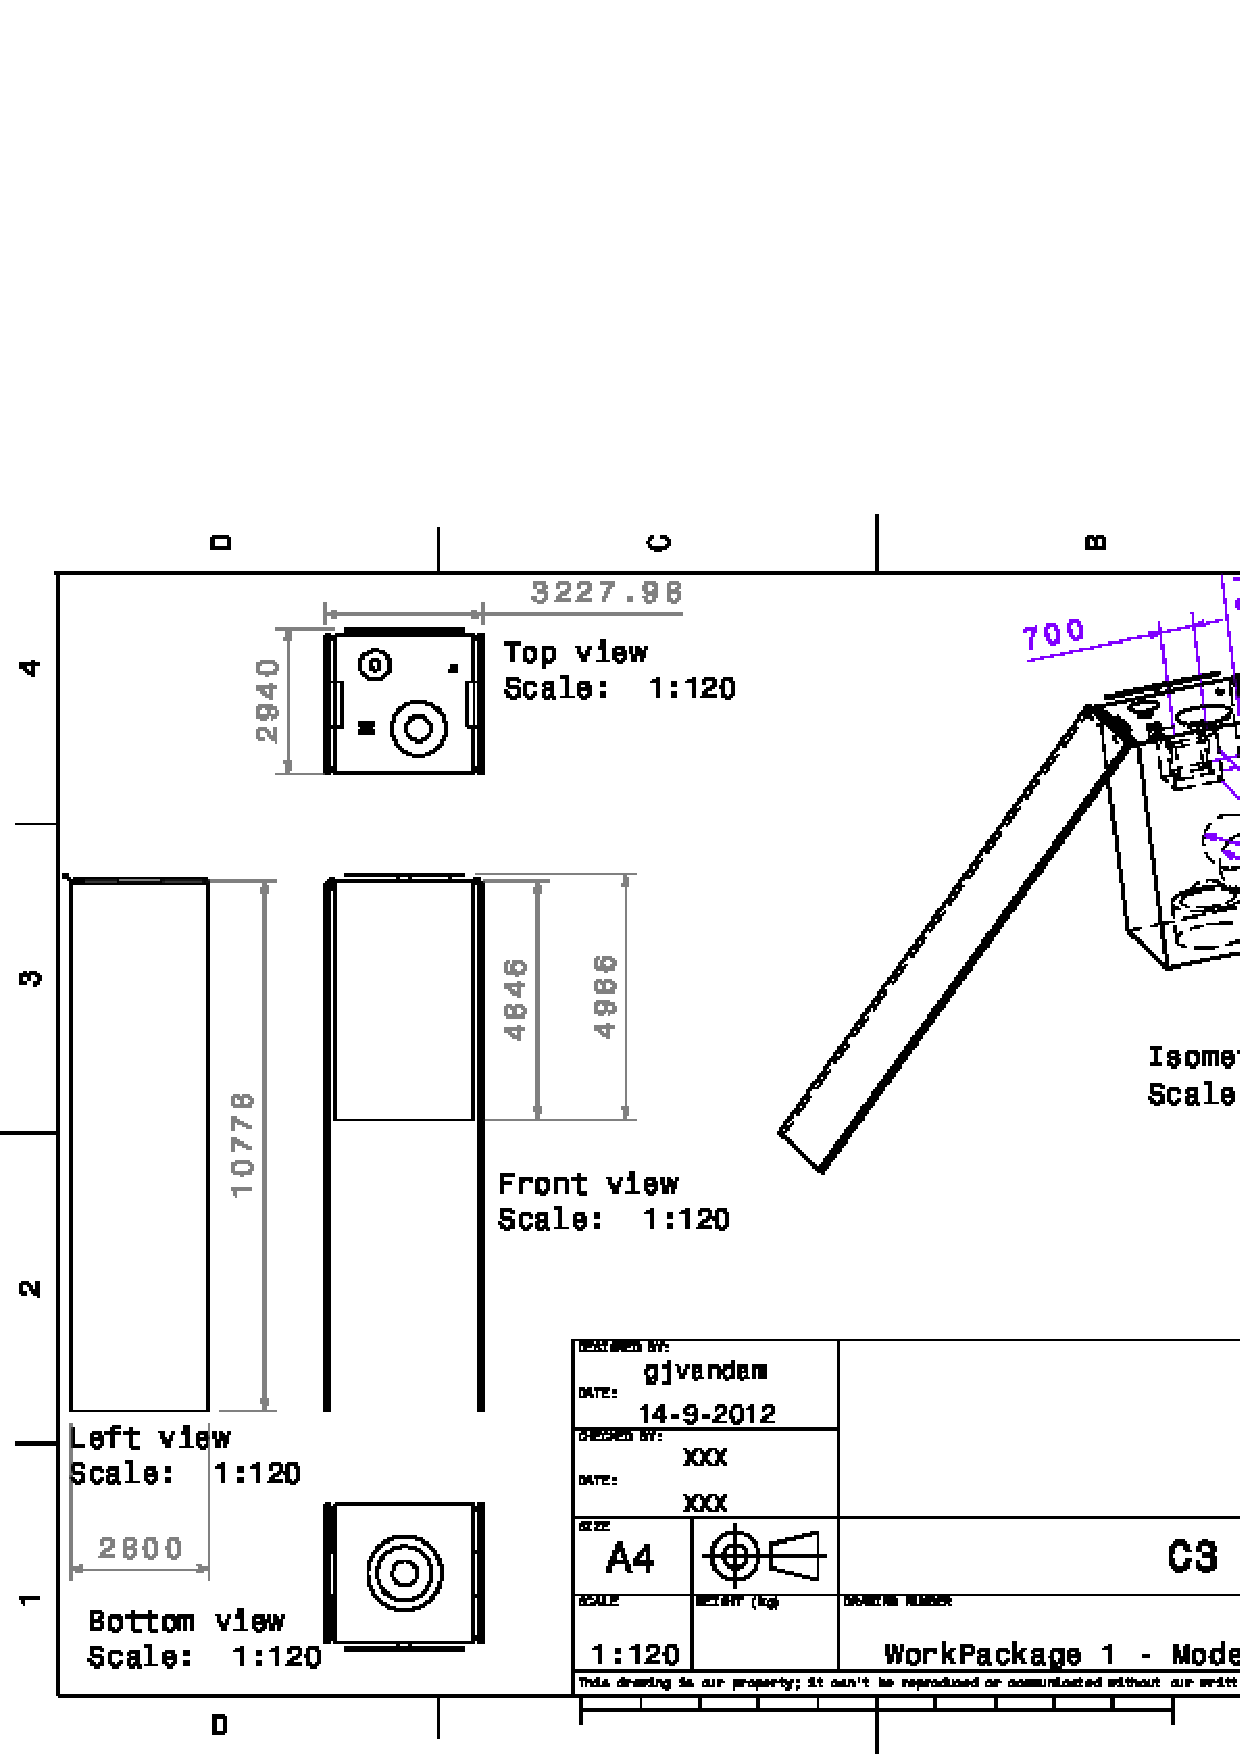
\includegraphics[angle=90, width=0.8\textwidth]{catiadraw1}
  \caption{catia drawing of a design}
  \label{sketch3-1}
\end{figure}

%% D1.4.4. Estimation of the vehicle MMOI in the deployed and
%% un-deployed state.

\deliverable{1.4.4}

In this section the Mass moments of Inertia of the different sketches
will be estimated.

%%maybe subsection

The first estimation will be about the cylindrical shape. The MMOI in
the direction of the height can be calculated by formula
\ref{MMOIcyl1}.

\begin{equation}
  \label{MMOIcyl1}
  \mathrm{MMOI}=\frac{1}{2}mr^2
\end{equation}
Every variable in this equation is known. the mass is \SI{3000}{kg},
the radius is \SI{1.75}{m}. This gives a MMOI of \SI{6000}{kgm^2}. The
MMOI on the other 2 axis is equal and can be calculated by using
formula \ref{MMOIcyl2}.

\begin{equation}
  \label{MMOIcyl2}
  \mathrm{MMOI}=\frac{1}{12}m(3r^2+l^2)
\end{equation}
Because the height of the satellite is also a known value, this can
also be found.  The MMOI is \SI{5286}{kgm^2}. Because the undeployed
state looks almost the same as the deployed state, the MMOI will not
change much if the satellite is deployed.

%%maybe add a subsection

For the MMOI of the cuboid perpendicular on the exhaust, formula
\ref{perpex} is used

\begin{equation}
  \label{perpex}
  \mathrm{MMOI}=\frac{1}{12}m(2.5^2+3.5^2)
\end{equation}
this gives a value of \SI{4625}{kgm^2}.

For the MMOI parallel to the side of length $3.5m$ formula \ref{mmoi35}

\begin{equation}
  \label{mmoi35}
  \mathrm{MMOI}=\frac{1}{12}m(2.5^2+4.4^2)
\end{equation}
This gives a MMOI of \SI{6400}{kgm^2}.

The MMOI parallel with the side of length \SI{2.5}{m} is calculated by
formula \ref{mmoi25}

\begin{equation}
  \label{mmoi25}
  \mathrm{MMOI}=\frac{1}{12}m(3.5^2+4.4^2)
\end{equation}
For this one, the MMOI is \SI{7900}{kgm^2}.

For the deployed MMOI of the cuboid shaped satellite, there are some
estimations needed for the solar panels. For these estimations, a
specific power is needed. This is \SI{25}{W/kg} for standard solar
panels. \cite{wertz1999space}

%% this citation is from the smad book
The solar array mass is then calculated by formula \ref{SpecificPower}

\begin{equation}
  \label{SpecificPower}
  M_a=\frac{P}{P_{sp}}=0.04*P
\end{equation}
This gives a solar array mass of \SI{19.4}{kg}.

Another needed value is the area offset. This is calculated by formula \ref{AreaOffset}

\begin{equation}
  \label{AreaOffset}
  L_a=\frac{3}{2}L+\frac{1}{2} \left(\frac{A_a}{2} \right)^{\frac{1}{2}}
\end{equation}

In formula \ref{AreaOffset} the L is the distance between the solar
arrays and the $A_a$ is the array surface. These are respectively
\SI{2.5}{m} and \SI{60}{m^2}. If those two values are inserted, an
area offset of $6.489 m$ is found. With these 2 values, the MMOI
caused by the solar panels can be calculated.

To clearify the axis sytem, it is shown in figure
\ref{axissystemcuboid}.

\begin{figure}[H]
  \centering
  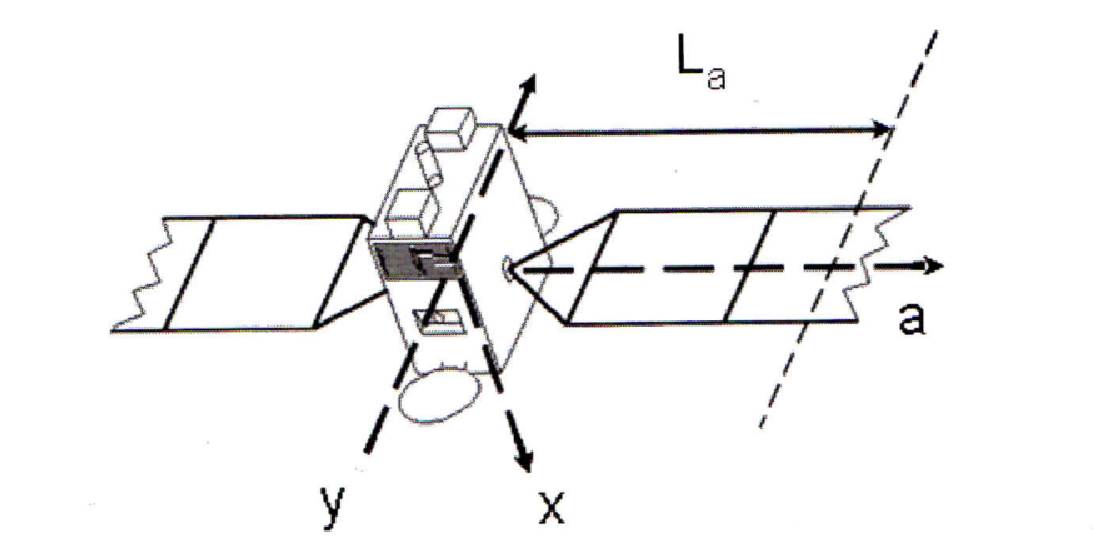
\includegraphics[width=\textwidth]{axissystem}
  \caption{axis sytem for calculating MMOI}
  \label{axissystemcuboid}
\end{figure}

For the MMOI perpendicular to the solar panel face, formula
\ref{mmoix} is used.

\begin{equation}
  \label{mmoix}
  \mathrm{MMOI}_x=\left(L_a^2+\frac{A_a}{12}\right)M_a
\end{equation}

This results in a moment of inertia of \SI{914}{kgm^2}.  For the MMOI
over the y-axis, formula \ref{mmoiy} is used.

\begin{equation}
  \label{mmoiy}
  \mathrm{MMOI}_y=\left(L_a^2+\frac{A_a}{24}\right)M_a
\end{equation}

This gives an MMOI of \SI{865}{kgm^2}.  For the MMOI around the
a-axis, formula \ref{mmoia} is used.

\begin{equation}
  \label{mmoia}
  \mathrm{MMOI}_a=\left(\frac{A_a}{24}\right)M_a
\end{equation}

Which gives a MMOI of \SI{49}{kgm^2}.

\begin{longtable}{rrrr}
\caption{summary of MMOI of cuboid shape} \\
 & undeployed & solar array & deployed \\
 MMOI$_x$ & 462 & 914 & 5539 \\
 MMOI$_y$ & 6400 & 865 & 7265 \\
 MMOI$_a$ & 7900 & 49 & 7949 \\
\end{longtable}
